% ==============================================================================================
\chapter{Moving load on an elastic halfspace} \label{ch:moving_load_halfspace}
% ==============================================================================================

% ----------------------------------------------------------------------------------------------
\section{Introduction}
% ----------------------------------------------------------------------------------------------
This benchmark compares the STEM numerical solution against the analytical solution,
for a moving load travelling on an elastic halfspace.

The analytical solution is presented in~\cite{Fryba_2013}.
The analytical solution provides closed-form expressions for the vertical displacement along the surface of the halfspace,
enabling a direct time-history comparison against the numerical model.

% ----------------------------------------------------------------------------------------------
\section{Model Description}
% ----------------------------------------------------------------------------------------------

% ..............................................................................................
\subsection{Geometry, mesh and loading}
% ..............................................................................................
The soil domain is modelled as a three-dimensional continuum representing a vertical column
with a height of \qty{10}{\meter} and a square cross-section of \qty{0.25}{\meter} by \qty{0.25}{\meter}.
The column is aligned with the $y$-axis, so that wave propagation is essentially one-dimensional along
the vertical direction.
The soil is discretised with high-order tetrahedral elements, using an average element size of \qty{0.10}{\meter}.
An overview of the geometry and mesh adopted for the analysis is shown in
Figure~\ref{fig:one_dim_wave_mesh}.
A vertical surface load is applied on the entire top face of the column. The load acts in compression along
the $y$-direction and is applied as a step function in time:

\begin{equation}
	p(t) =
	\begin{cases}
		0, & t < \qty{0}{\second}, \\
		\qty{-1000}{\kilo\newton\per\meter\squared}, & t \geq \qty{0}{\second}.
	\end{cases}
\end{equation}

The base of the column is fully fixed, preventing displacements in all three directions.
The four vertical faces are restrained only in the horizontal directions, thereby allowing vertical motion
similar to an one-dimensional situation.

\begin{figure}
	\centering
	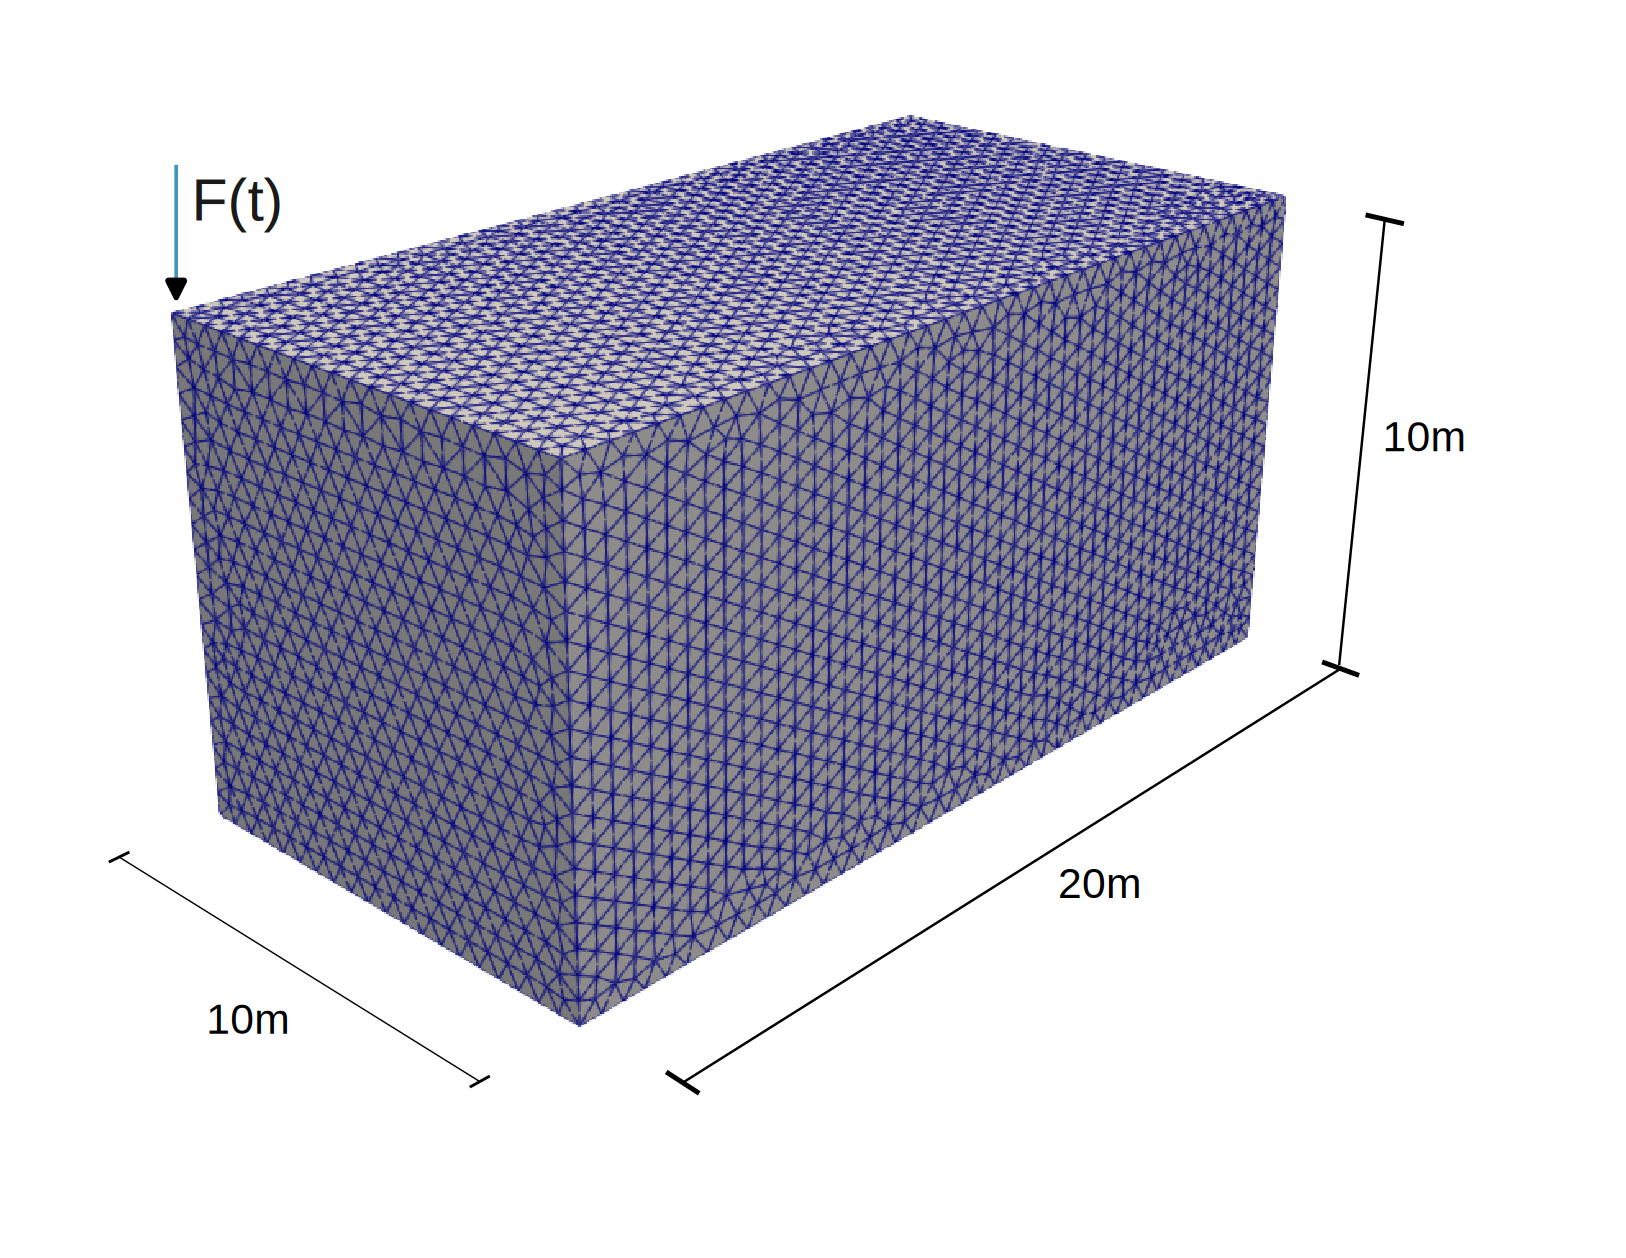
\includegraphics[width=0.75\textwidth]{one_dim_wave_prop/mesh.pdf}
	\caption{Geometry, mesh and boundary conditions adopted for the one-dimensional
	wave propagation benchmark.}
	\label{fig:one_dim_wave_mesh}
\end{figure}

% ..............................................................................................
\subsection{Materials and numerical parameters}
% ..............................................................................................
The soil is modelled as an one-phase continuum with a linear elastic constitutive law, with the
following parameters:

\begin{itemize}[noitemsep,topsep=0pt,parsep=0pt,partopsep=0pt]
	\item Young's modulus: \qty{50}{\mega\pascal},
	\item Poisson ratio: \qty{0.3}{},
	\item Solid density: \qty{2700}{\kilogram\per\meter\cubed},
	\item Porosity: 0.3.
\end{itemize}


Material damping is included via Rayleigh damping, with parameters that provide a damping ratio of
\qty{0.5}{\percent} at \qty{1}{\hertz} and \qty{80}{\hertz}.

The dynamic analysis is performed over a \qty{0.20}{\second} time window, with a time step of \qty{0.001}{\second}.
The system of equations is solved using the Newmark time integration~\cite{Newmark_1959} scheme with
parameters $\beta = 0.25$ and $\gamma = 0.5$.


% ----------------------------------------------------------------------------------------------
\section{Results}
% ----------------------------------------------------------------------------------------------
Figure~\ref{fig:one_dim_wave_results} presents the time histories of the
vertical velocity at three points located at: \qty{2.5}{\meter}, \qty{5}{\meter} and \qty{7.5}{\meter}
along the height of the column.
The figure compares the numerical STEM results against the analytical solution of the one-dimensional wave equation.

The arrival times of the incident and reflected waves at the observation point match closely between the numerical
and analytical solutions.
The amplitudes of the displacement and velocity pulses also show very good agreement, with small differences
attributable to the introduced material and numerical damping.

\begin{figure}[h]
	\centering
	\includegraphics[width=0.8\textwidth]{one_dim_wave_prop/time_history.pdf}
	\caption{Comparison of the vertical velocity time histories at three points located at:
    (a) \qty{2.5}{\meter}, (b) \qty{5}{\meter} and (c) \qty{7.5}{\meter}
	along the column height.}
	\label{fig:one_dim_wave_results}
\end{figure}

